\chapter{Transferencia de carga en complejos colorante-SC utilizando un modelo TB.}

La conversión eficiente de la energía solar en formas utilizables es uno de los desafíos científicos y tecnológicos más importantes de este decenio. El desarrollo de nuevos materiales y técnicas de captación de energía solar requieren de la convergencia de múltiples disciplinas en un objetivo común. Desde el punto de vista de la simulación computacional los aportes que pueden ser realizados en este campo implican el desarrollo y aplicación de técnicas capaces de predecir las propiedades ópticas de nuevos materiales complejos. 

Las DSSC dado su bajo costo y robustez en relación a otras tecnologías de captación de luz solar, pueden potencialmente reemplazar a las fuentes de energía tradicionales. El paso principal en el proceso de fotoinyección de las DSSC, es la transferencia de electrones desde el colorante al SC. Si bien las simulaciones atomı́sticas dan una figura muy completa del proceso de transferencia de carga y permiten predecir el mecanismo para un colorante arbitrario, no tenemos aún una comprensión de cuáles son los parámetros fundamentales en la determinación del mecanismo. 

El presente capítulo pretende dar un paso más en la profundidad de comprensión a partir del desarrollo de un modelo simple que nos permita tener una visión muy simplificada pero con los ingredientes cruciales que determinan el mecanismo de transferencia de carga. El objetivo es desarrollar un modelo capaz de describir todo el espectro de situaciones y predecir el mecanismo de transferencia a partir de las propiedades del colorante y del SC sin necesidad de llevar a cabo simulaciones atomı́sticas ni experimentos.


\section{Modelo TB}

Para llevar a cabo el objetivo planteado se utilizó un modelo TB simple para describir la dinámica de fotoinyección en complejos colorante-SC no periódicos y para ello fue necesario, en primera instancia, representar teóricamente una molécula adsorbida a un SC. Es importante recalcar que en este modelo, se utiliza una molécula diatómica para modelar simplificadamente el colorante. 

Para simular la molécula diatómica se utilizó un sistema de dos niveles (TLS, en inglés: Two Level System) que reproducen los orbitales HOMO-LUMO (H-L). El TLS ha sido muy utilizado desde los comienzos de la mecánica cuántica ya que reproduce de manera realista la interacción entre un ́atomo o molécula con un campo electromagnético emitido por un láser, y asimismo, la dinámica del TLS interaccionando con un campo externo es uno de los pocos modelos de este tipo que presentan una solución exacta.


Para representar la estructura electrónica del SC se utilizó un anillo finito de átomos con distorsiones periódicas para introducir el GAP, generadas con distancias interatómicas alternadas de manera que la interacción de cada uno de los ́atomos sea distinta con cada uno de sus dos vecinos próximos. Para entender la teoría que explica el anillo distorcionado es necesario comenzar con modelos más simples, por ejemplo el modelo de banda s donde se asocia un estado s a cada átomo y como resultado se obtiene una sola banda de estados. Un ejemplo para este modelo son moléculas hipotéticas que consisten de cadenas de átomos de H. Tales cadenas no existen en realidad debido a que no son energéticamente favorables, sin embargo, existen algunas moléculas cadena muy importantes que se forman agregando unidades como es el caso de los alcanos y alquenos. A pesar de que la estructura electrónica de estos últimos es mucho más complicada con respecto a las cadenas de H, existe una gran similitud sobre como se configuran los cálculos. La desventaja que tiene este sistema radica en el hecho de que los átomos en el \textit{bulk} de la cadena lineal ignoran lo que ocurre en los átomos finales. Una solución a este inconveniente resulta de cerrar la cadena en sí misma hasta formar un anillo ya que de esta manera eliminamos los ``átomos superficiales'' que se encuentran al final de la cadena y todos los átomos en el anillo son equivalentes. La figura \ref{anillo_equi} muestra el anillo de átomos de H, donde cada átomo está asociado a un estado s y asumimos que el set de estados sobre los N átomos de H forma una base completa en la cuál expandir el estado molecular \cite{sutton}.

\begin{figure}[!htb]
\centering
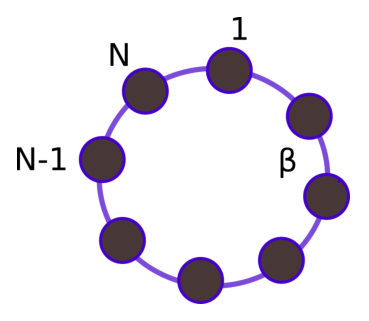
\includegraphics[height=4cm]{cap3/figs/ring_nodist_solo.eps}
\caption{Anillo de N átomos de H.} 
\label{anillo_equi}
\end{figure}

\newpage

Utilizando $c_j= e^{ij\theta}$ e incluyendo la constante de normalización $\frac{1}{N^{1/2}}$ obtenemos:

\begin{equation}
\ket \Psi = \frac{1}{N^{1/2}} \sum_{j=1}^N e^{ij\theta} \ket j
\label{eq:molecular}
\end{equation}

donde el estado s sobre el átomo j se representa con el ket $\ket j$ y el número cuántico $\displaystyle \theta = \frac{2m\pi}{N}$ donde m = 0,1,2,...,(N-1). La ecuación \ref{eq:molecular} es una función de Bloch y se deriva de la simetría traslacional del anillo, en otras palabras, todos los átomos en el anillo son equivalentes por una simple traslación alrededor del anillo. Los valores permitidos de $\theta$ derivan de la periodicidad del estado molecular, es decir, c$_N$ = c$_0$ y c$_{N+1}$ = c$_1$. 

Insertando la ecuación \ref{eq:molecular} en la ecuación de Schr\"odinger $H \ket \Psi = E \ket \Psi $, obtenemos:

\begin{equation}
\sum_{j=1}^N e^{ij\theta} H \ket j = E \sum_{j=1}^N e^{ij\theta} \ket j
\end{equation}

y multiplicando por la izquierda el bra $\bra p$ obtenemos:

\begin{equation}
\sum_{j=1}^N e^{ij\theta}  \bra p H \ket j = E \sum_{j=1}^N e^{ij\theta} \langle p \ket j
\end{equation}

Donde $\langle p \ket j = 0$ excepto cuando $j=p$ asumiendo que la base es ortonormal, entonces:


\begin{equation}
\sum_{j=1}^N e^{ij\theta}  \bra p H \ket j = E e^{ip\theta}
\end{equation}

o, tomando el factor $e^{ip\theta}$ en el lado izquierdo de la igualdad:

\begin{equation}
\sum_{j=1}^N e^{i(j-p)\theta}  \bra p H \ket j = E({\theta})
\end{equation}

Los elementos de matriz $\bra p H \ket j$ son nulos excepto cuando $j=p$ o $j = p+1$ o $j = p-1$. Cuando $j=p$ obtenemos los elementos de matriz \emph{on site} $\bra p H \ket j = \alpha$ y cuando $j = p+1$ o $j = p-1$ obtenemos los elementos de matriz entre átomos vecinos (integrales de \emph{hopping} o simplemente \emph{hopping}) $\bra p H \ket j = \beta$. Entonces hay solo 3 términos en la suma de la izquierda que no son nulos:

\begin{equation}
\alpha + \beta e^{i\theta} + \beta e^{-i\theta} = \alpha + 2\beta \cos{\theta} = E
\end{equation}

En cristales de una dimensión (1D) el GAP es introducido por distorciones periódicas llamadas distorciones de Peierls. Considerando un anillo de átomos equiespaciados (distancia = a) y \emph{hopping} $\beta$ generamos la banda prohibida al mover los átomos del anillo con el objetivo de generar 2 distancias interatómicas alternadas (a y b) y por ende 2 \emph{hopping} $\beta_1$ y $\beta_2$ como se muestra en la figura \ref{anillo_dist}. Las distorciones de Peierls se asemejan a una molécula de poliacetileno donde se intercalan enlaces simples y dobles. 

\begin{figure}[!htb]
\centering
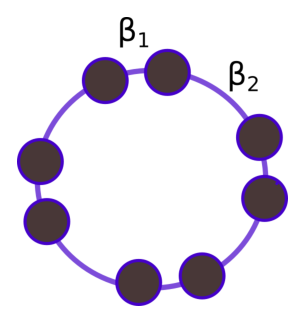
\includegraphics[height=4cm]{cap3/figs/ring_dist_solo.eps}
\caption{Anillo distorcionado con hopping electrónicos $\beta_1$ y $\beta_2$.} 
\label{anillo_dist}
\end{figure}

El complejo en cuestión simulado con un modelo TB es el que se muestra en la figura \ref{anillo_dist_mol}. El anillo puede acoplarse en distintos grados a una molécula diatómica, lo cual está regulado por el parámetro $\gamma$. La interacción entre los ́atomos de la molécula se representa con el parámetro $\delta$, por lo que la transición electrónica tiene una energía de 2 $\delta$. El centro de energía de la diatómica respecto al centro del GAP del semiconductor está representado por el parámetro $\epsilon$. Los \emph{hopping} electrónicos $\beta_1$ y $\beta_2$ son una medida de las interacciones entre los átomos del anillo y por esta razón regulan el GAP. Por último, otro de los parámetros que se tiene en cuenta a la hora de la simulación, es $\mu$, el cual define el potencial electroquímico de los electrones en todo el sistema con una temperatura tal que $kT = 0.001$ Ha.

\begin{figure}[!htb]
\centering
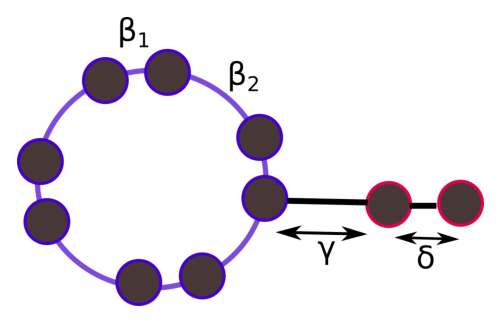
\includegraphics[height=4cm]{cap3/figs/ring_dist.eps}
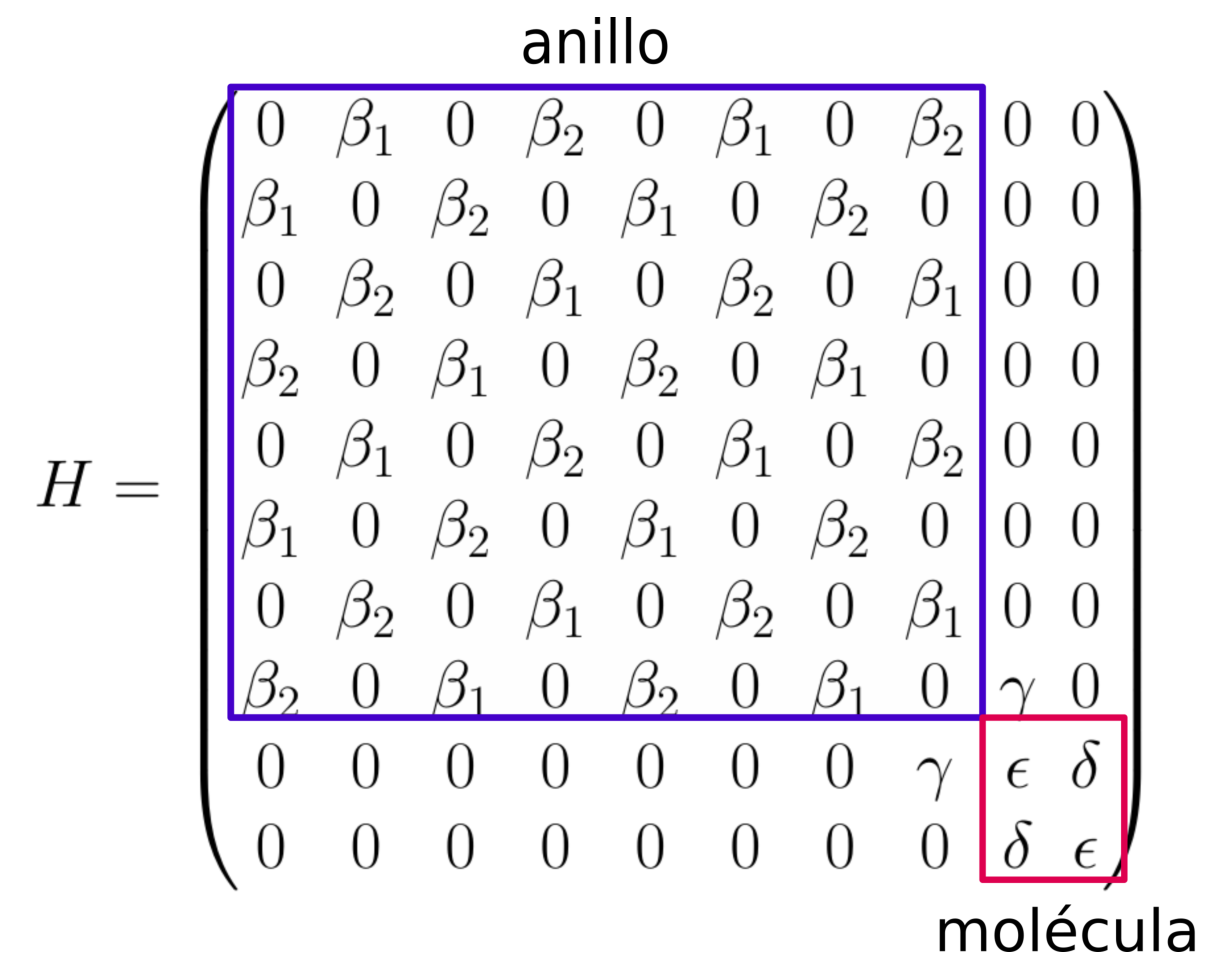
\includegraphics[height=4.5cm]{cap3/figs/h_1.eps}
\caption{\textbf{Izquierda} Esquema del anillo semiconductor acoplado a una diatómica. \textbf{Derecha} hamiltoniano para un sistema N=10.} 
\label{anillo_dist_mol}
\end{figure}

El hamiltoniano modelo es de electrones independientes y por tanto desprecia completamente los efectos de las interacciones inter-electrónicas, tanto de intercambio como coulómbicas. La inclusión de interacción electrón-electrón a campo medio (en un modelo autoconsistente) será objeto de un trabajo posterior. El efecto fundamental de la interacción electrón-electrón en estos sistemas, en base a la experiencia adquirida en el grupo en los últimos años, se reduce a una renormalización de las energías de excitación y velocidades de transferencia electrónica. Dado que el objetivo del modelo es lograr una descripción cualitativa del fenómeno se priorizó la simplicidad del hamiltoniano para facilitar la comprensión de los resultados y posibilitar una exploración extensiva del espacio de parámetros. Es importante aclarar que no se tiene en cuenta la disipación térmica de los núcleos, en este modelo sólo se considera el movimiento electrónico.

El hamiltoniano fue calculado a través de una matriz NxN (N = número de atomos del sistema) con dos bloques principales, uno que representa al SC y otro a la molécula. En la figura \ref{anillo_dist_molohenberg1964} a la derecha se muestra el hamiltoniano cuando N = 10. El bloque del hamiltoniano correspondiente al SC tiene dimensiones N-2 x N-2 con elementos de matriz nulos cuando i = j $\pm$ 2n mientras que para i= j+(2n $\pm$ 1) se muestran los \emph{hopping} de forma alternada.

El bloque de la diatómica tiene dimensiones 2x2 debido a los orbitales H-L. El parámetro $\epsilon$ conforma la diagonal y en el resto del bloque se encuentra $\delta$. El acoplamiento, $\gamma$, se encuentra en H$_{N−2,N−3}$ y H$_{N−3,N−2}$, entre los dos bloques.

\subsection{Cálculo de la densidad de estados}

Suponiendo que tenemos todos los autoestados $\ket n$ y las energías E$_n$ de un hamiltoniano electrónico simple, se define a la densidad total de estados para un sistema finito DOS(E) por la relación: 

\begin{equation}
\label{dos_finito}
\displaystyle DOS (E) = \sum_n \frac{1}{\sqrt{2}}  e^{\frac{(E-E_n)^ 2}{\sigma^2}}
\end{equation}

donde $\sigma$ es el ancho de una función gaussiana.

Esto debe entenderse en el sentido operacional, que si integramos la DOS(E) sobre un rango de energía, obtenemos el número total de estados dentro del mismo \cite{finnis}. Para sistemas infinitos la densidad de estados se calcula mediante funciones delta de Dirac pero cuando se trata de sistemas finitos, como el planteado en el presente capítulo, se ensanchan las deltas de Dirac utilizando funciones gaussianas para cada una de las energías.


\subsection{Cálculo del espectro de absorción}

La expresión general de la función respuesta lineal para un gas de electrones no interactuantes \cite{giuliani}: 

\begin{equation}
\label{espectro_general}
\chi_{AB}^{(0)} = \sum_{\alpha\beta} \frac{n_\alpha- n_\beta}{\hbar+ \epsilon_\alpha- \epsilon_\beta + i\hbar\eta} A_{\alpha \beta} B_{\beta \alpha}
\end{equation}

donde $n_\alpha$ y $n_\beta$ es la ocupación promedio Fermi-Dirac del estado $\alpha$ y el estado $\beta$, respectivamente a temperatura T y potencial electroquímico $\mu$ de los electrones, $\epsilon$$_\alpha$– $\epsilon$$_\beta$ es la diferencia de energía entre los estados $\alpha$ y $\beta$ y A$_{\alpha \beta}$, B$_{\beta \alpha}$  son los elementos de matriz de los operadores A y B. 

A los fines de describir el espectro de absorción, se calculó la función de respuesta lineal, donde los operadores A y B son en este caso, los operadores momento dipolar de transición $\mu$$_{\alpha\beta}$ y $\mu$$_{\beta\alpha}$ (ver ecuación \ref{espectro}) los cuales otorgan el peso a la transición.

Los términos $n$$_\alpha$ y $n$$_\beta$ indican que cuando los estados $\alpha$ y $\beta$ están ambos ocupados o desocupados, el numerador de la ecuación es cero y por ende también el término de la sumatoria. De esta forma, las únicas transiciones que se toman en cuenta a la hora del cálculo del espectro, son las de estado ocupado a desocupado.

\begin{equation}
\label{espectro}
\chi_{\mu_{\alpha\beta} \mu_{\beta \alpha}}^{(0)} = \sum_{\alpha\beta} \frac{n_\alpha- n_\beta}{\hbar+ \epsilon_\alpha- \epsilon_\beta + i\hbar\eta} {\mid{{\mu _{\alpha\beta}}}\mid} ^{2}
\end{equation}
 
\subsection{Cálculo de transferencia de carga}

Para estudiar la transferencia de carga fue necesario calcular la dinámica electrónica del sistema bajo la acción de un láser.  Se procedió, en primera instancia, a diagonalizar el hamiltoniano para calcular la matriz de autovectores y de esa forma calcular el operador matriz densidad monoelectrónica $\hat{\rho}$. Para realizar el cálculo de la transferencia de carga se aplica una perturbación con forma de función sinusoidal $E(t) = E_0 \sen{(\omega t)}u$, donde $E_0$ es la intensidad del campo y $\omega$ la frecuencia de excitación de interés. 

Cuando se perturba a partir de t = 0 el operador $\hat{\rho}$, se inicializa la dinámica. La integración numérica para obtener la propagación electrónica se realiza a partir del algoritmo:

\begin{equation}
 \label{leapfrog}
  \hat{\rho}(t+\delta t) = \hat{\rho}(t-\delta t) + 2 \delta t \frac{\partial \hat{\rho}(t)}{\partial t}  
\end{equation}

donde $\hat{\rho}(t + \delta t)$ es el operador matriz densidad propagado en el tiempo, $\hat{\rho}(t - \delta t)$ es el operador matriz densidad en el paso anterior y $\frac{\partial \hat{\rho}(t)}{\partial t}$ es la derivada parcial del operador matriz densidad con respecto al tiempo, este último se obtiene a partir de la ecuación de Liouville-von Newmann:

\begin{equation}
 \label{newman}
  \frac{\delta \hat{\rho}}{\delta t}= \frac{1}{i\hbar} (\hat{H}\hat{\rho} - \hat{\rho}\hat{H})
\end{equation}


donde $\hat{\rho}$ es el operador matriz densidad y $\hat{H}$ es el operador Hamiltoniano.

En este caso la intensidad del campo llevó al sistema fuera del régimen de respuesta lineal, ya que se buscó sacar al sistema del equilibrio y ver el posible movimiento de los electrones en el tiempo. Luego del cálculo de la dinámica se procede a analizar/graficar la variación de las poblaciones electrónicas con respecto al tiempo ya que de esta forma podemos observar indirectamente la transferencia de carga.

\section{Simulación de complejos colorante-SC utilizando el modelo propuesto.}

Utilizando el modelo propuesto se calcularon y estudiaron: densidad de estados o DOS, espectros de absorción y transferencia de carga en complejos diatómica-anillo. Para llevar a cabo dichas tareas fue necesario variar uno o varios de los parámetros del modelo mientras los restantes se mantuvieron constantes y luego se analizó el comportamiento del sistema en respuesta a los cambios que se generaron. De esta forma, se realizó el procedimiento con cada uno de los parámetros de interés para obtener una mirada general del modelo bajo estudio.

A través de investigaciones que se realizaron en el grupo, se conoce que los SC utilizados en las DSSC tienen un GAP de aproximadamente 3 eV (zona del ultravioleta) mientras que el colorante, como absorbe en el visible, tiene una diferencia energética H-L promedio de 2 eV. Con el fin de que el modelo represente situaciones lo más reales posibles, se tomaron ciertos valores para los parámetros que respeten la relación $\frac{3}{2}$ de energía de absorción entre el SC y la molécula diatómica. Por ello, a lo largo de todo del capítulo, se utilizaron los valores de \emph{hopping} electrónicos $\beta_1= -0.5$ y $\beta_2= -1.0$ para el SC que definen un GAP de 1 u.a. de acuerdo a la relación $ GAP = 2\mid{\alpha-\beta}\mid$ y $ 2\delta = -0.6$ como valor de energía necesaria para la transición de la diatómica.

Los parámetros que se fueron modificando para realizar el análisis fueron: $\epsilon$ ya que posiciona energéticamente los orbitales HOMO-LUMO de la diatómica con respecto al centro del GAP del SC, $\mu$ que determina el potencial electroquímico de los electrones en el sistema y $\gamma$ que establece el acoplamiento entre la molécula y el SC.


\subsection{Sistema sin acoplamiento}

Una molécula pueda considerarse un buen sensibilizador en una DSSC si cumple con diversos requisitos, entre otros, que absorba en la región visible del espectro e incluso en el infrarrojo cercano. En las DSSC más comunes (por ejemplo las celdas de Gr\"atzel \cite{ORegan1991}) el LUMO o nivel de energía del estado excitado del fotosensibilizador debe ser mayor en energía que la energía del borde de la banda de conducción (BC) del semiconductor (SC). También se ha demostrado la existencia de DSSC en las que el HOMO del colorante se encuentra ubicado energéticamente en la BV del SC \cite{Negre2014,Borgstrom2005}.
 
Como punto de partida, se consideró el sistema colorante - SC sin acoplamiento, dicho de otro modo, {\bf $\gamma=0$}, para corroborar la eficacia del modelo en un amplio espectro de situaciones. Tomando $\gamma$ como parámetro fijo, se utilizaron valores de $\epsilon$ y $\mu$ tal que garanticen 2 situaciones particulares: \textbf{(1-e)} el LUMO de la molécula se encuentre energéticamente dentro de la BC del SC y \textbf{(1-h)} el HOMO de la molécula se encuentre energéticamente dentro de la banda de valencia (BV) del SC. Para evaluar el sistema \textbf{(1-e)} se utilizaron los parámetros $\epsilon=0.45$ y $\mu=0.3$ y para el sistema \textbf{(1-h)} se utilizaron los parámetros $\epsilon=-0.45$ y $\mu=-0.3$

\begin{figure}[!htb]
 \centering
 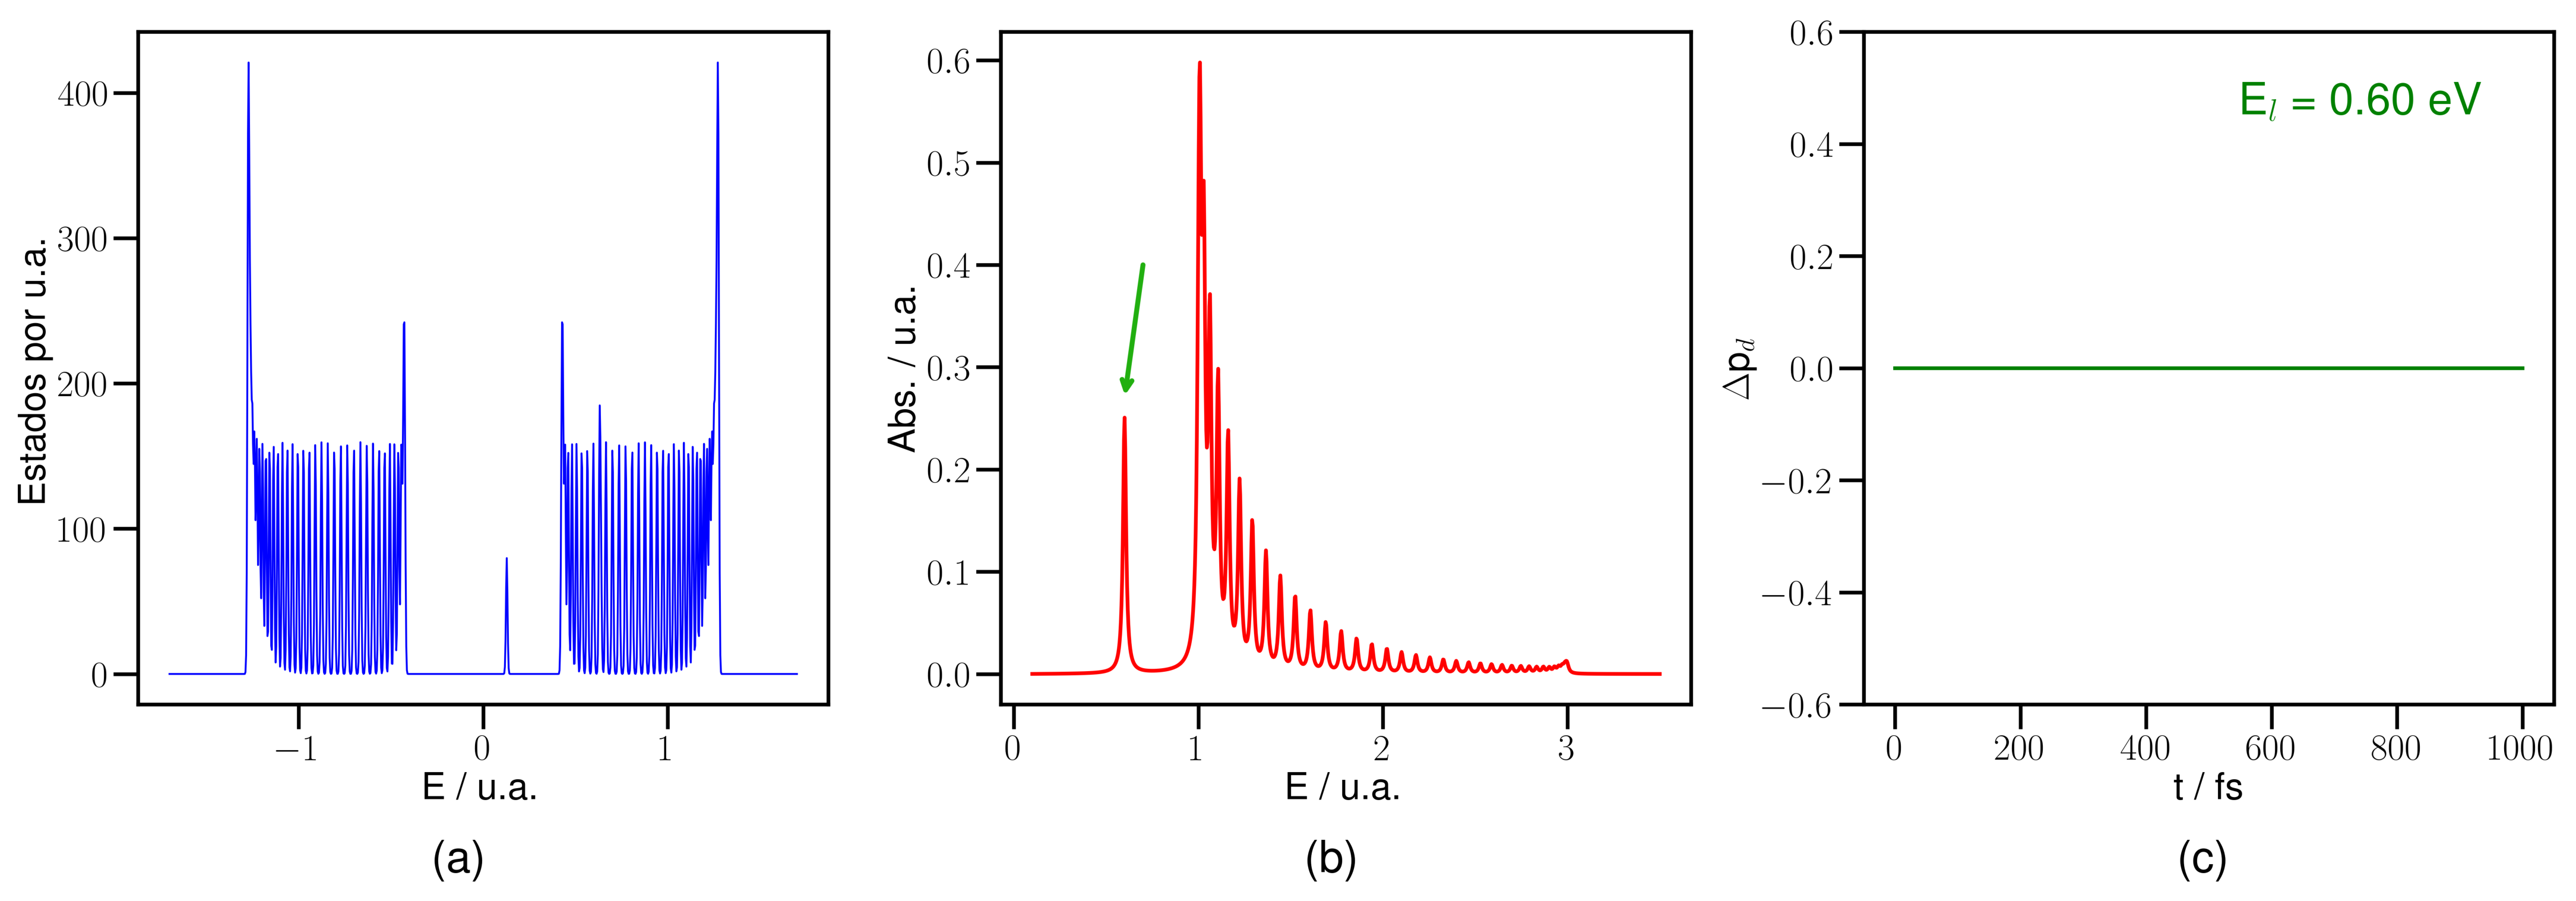
\includegraphics[height=5cm]{cap3/figs/fig_s_acople_diat.eps}
 \caption{Sistema \textbf{(1-e)}. \textbf{(a)} DOS, \textbf{(b)} espectro de absorción y \textbf{(c)} diferencia de población en la diatómica respecto a la población inicial ($\Delta p_d$) en función del tiempo aplicando un campo electromagnético con energı́a $0.6$ u.a.}
 \label{1-e}
\end{figure}


Los gráficos de la figura \ref{1-e} corresponden a los resultados para los cálculos del sistema \textbf{(1-e)}. En el gráfico de la DOS {\textbf{(a)} se observa por un lado el HOMO de la diatómica a $0.15$ u.a. de acuerdo al parámetro $\delta = 0.3$ elegido. El LUMO no se observa a simple vista debido a que se encuentra energéticamente dentro de la BC. Por otro lado, las 2 bandas del SC, a menor energía la BV y a mayor energía la BC separadas por un GAP de 1 u.a. Se puede observar también el nivel de Fermi en cero, entre la BV y BC, que junto con el GAP representan los parámetros típicos de un SC. Como el mismo posee bandas (a diferencia de la molécula), tiene una gran cantidad de estados disponibles para las transiciones.

El espectro de absorción del sistema con acoplamiento nulo \textbf{(b)} muestra un pico a aproximadamente $0.6$ u.a. de intensidad moderada y una banda a mayor energía en el rango $1-1.5$ u.a. con una intensidad mayor. Como ya se mencionó anteriormente, la diatómica puede solamente sufrir transiciones entre los orbitales H-L mientras que en el SC cualquier electrón que cuente con la energía necesaria puede excitarse desde la BV a la BC, por ello el pico del espectro corresponde a la absorción de la molécula y la banda al SC. La energía necesaria para que ocurra la transición H-L de la diatómica es mucho menor que la requerida para que ocurra la transición BV-BC del SC. Este comportamiento se debe a que la relación $\frac{3}{2}$ entre las energías de absorción de la diatómica y el SC se corresponde con DSSC reales en las que el colorante aislado absorbe en el visible y el SC aislado en el ultravioleta (por ejemplo complejos colorante-TiO$_2$). La energía necesaria para que ocurra una transición en el visible es menor que la necesaria para que ocurra en el ultravioleta, lo cual se encuentra plasmado en el espectro. Tambien se observa en la banda del SC, picos con distintas intensidades. La transición que genera la máxima intensidad en el espectro es la que ocurre desde el último nivel de energía de la BV al primer nivel de energía de la BC porque es el proceso menos energético mientras que los picos menos intensos son producto de transiciones que requieren más energía. Contribuye también a la intensidad de los picos el hecho de que las densidades de estado al borde de banda son máximas.

Para estudiar la transferencia de carga del sistema \textbf{(1-e)} sin acoplamiento fue necesario aplicar una perturbación continua de tipo láser con la energı́a de la transición de interés. Los parámetros utilizados para la dinámica electrónica fueron: paso de tiempo $0.01$ fs, número de pasos 100000 e intensidad del campo aplicado $0.01$ V /$\AA$. Como se mencionó anteriormente, la transferencia de carga se deduce indirectamente a través del gráfico de la evolución temporal de la población electrónica en la molécula diatómica ($\Delta p_d$) a medida que se perturba con el láser. 

En la figura \ref{1-e} {\textbf{(c)} se muestra $\Delta p_d$ en función del tiempo al iluminar el complejo molécula-SC con un láser sintonizado con la energía H-L de la diatómica ($0.6$ u.a.). En este caso los electrones de la molécula no se transfieren al SC, en otras palabras, no se observa transferencia de carga neta debido al acoplamiento nulo entre los mismos. En su lugar hay movimiento de electrones al perturbar con las distintas frecuencias de absorción.

\begin{figure}[!htb]
 \centering
 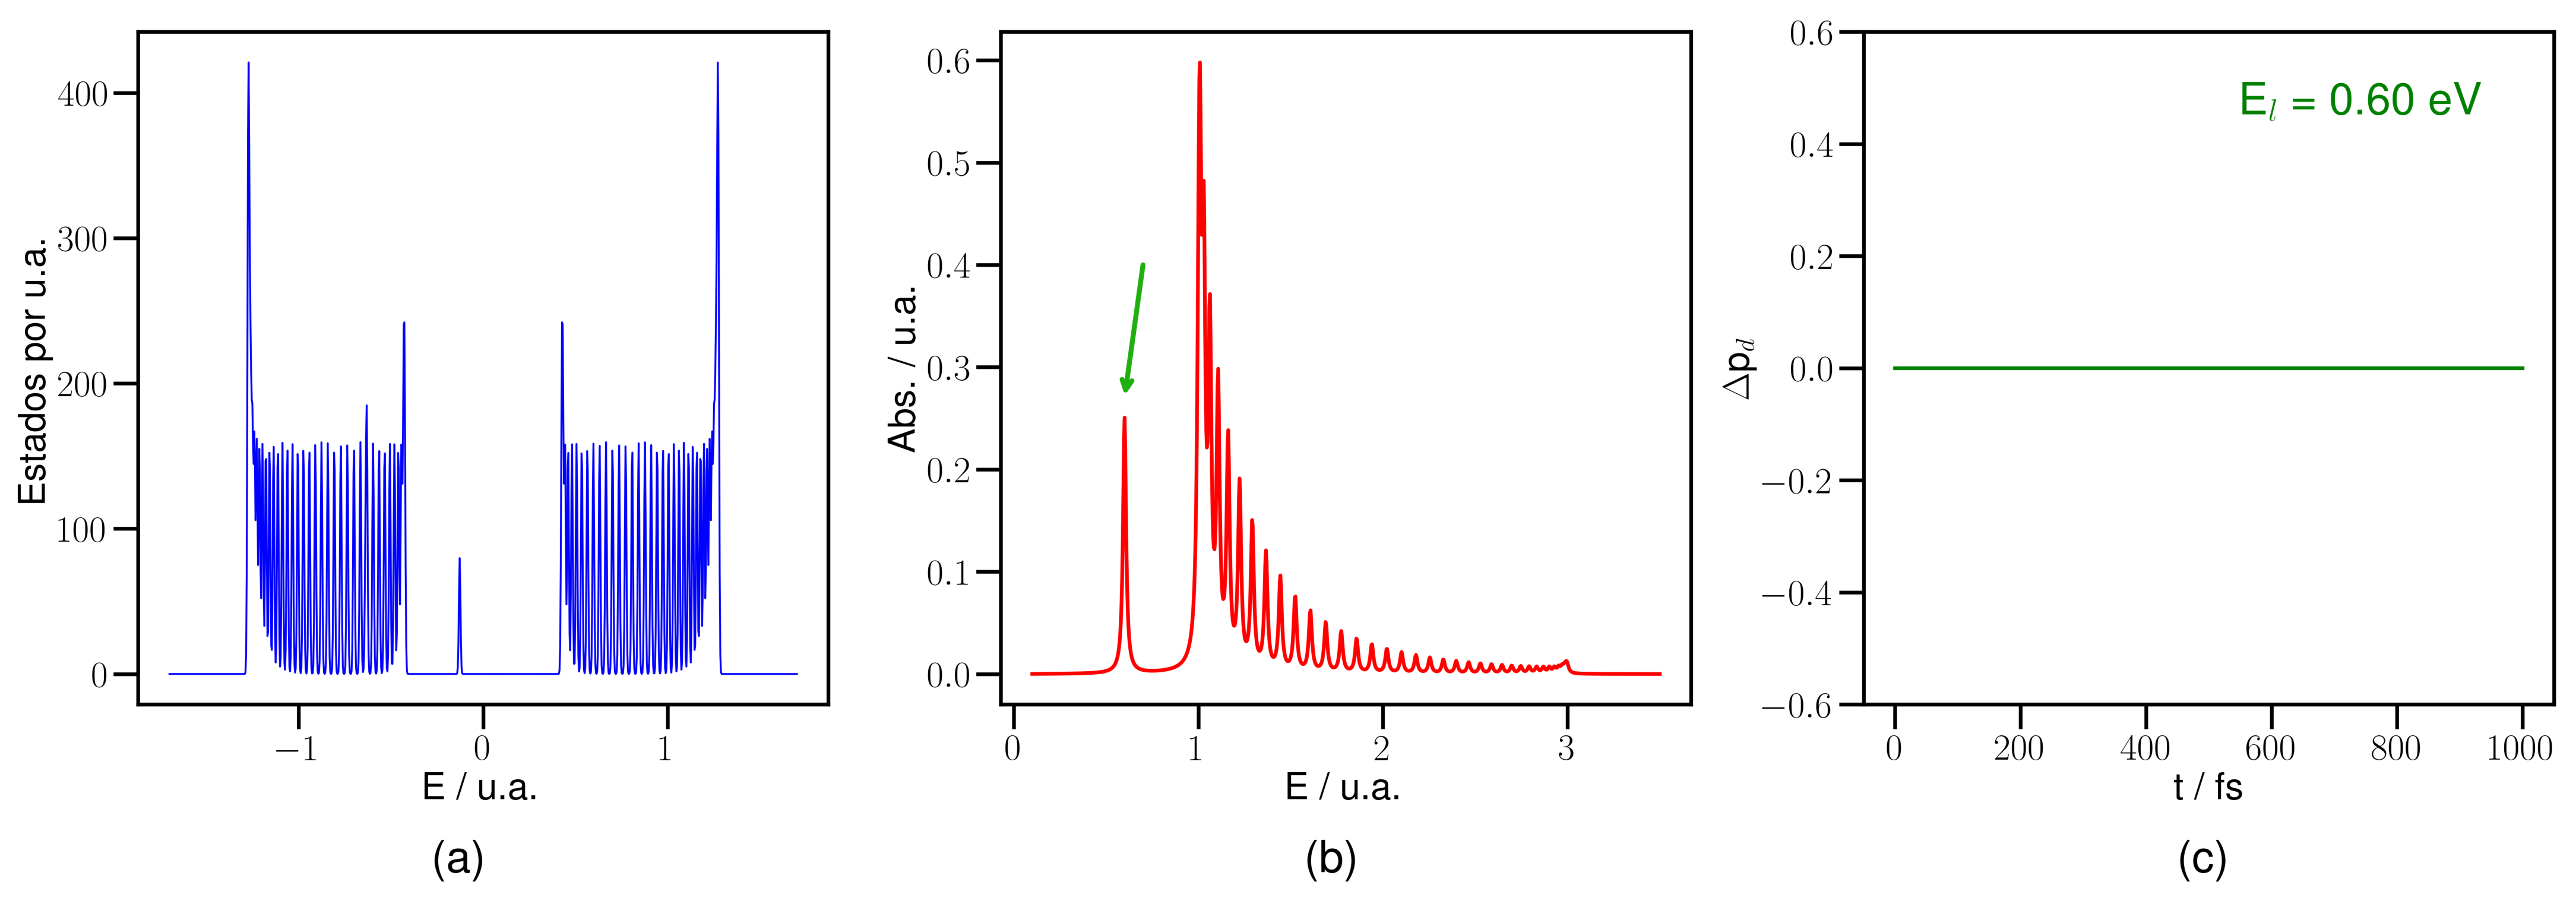
\includegraphics[height=5cm]{cap3/figs/fig_s_acople_diat_hueco.eps}
 \caption{Sistema \textbf{(1-h)}. \textbf{(a)} DOS, \textbf{(b)} espectro de absorción y \textbf{(c)} diferencia de población en la diatómica respecto a la población inicial ($\Delta p_d$) en función del tiempo aplicando un campo electromagnético con energı́a $0.6$ u.a.}
 \label{1-h}
\end{figure}

Los gráficos de la figura \ref{1-h} corresponden a los resultados para los cálculos del sistema \textbf{(1-h)}. En este caso los gráficos de \textbf{(b)} y \textbf{(c)} permanecen iguales al sistema \textbf{1-e}. El cambio en los parámetros $\epsilon$ y $\mu$ afecta a la molécula diatómica y se ve reflejado en el gráfico de la DOS \textbf{(a)}. A diferencia del sistema \textbf{(1-e)} se observa el LUMO de la molécula a $-0.15$ u.a. debido a que el HOMO se encuentra energéticamente dentro de la BC. El pico de la diatómica en el espectro de absorción \textbf{(b)} se encuentra también a $0.6$ u.a. ya que el parámetro $\delta$ que determina la energía de excitación H-L se conserva y la transferencia de carga sigue siendo cero por el acoplamiento nulo. 

%\newpage

\subsection{Sistema con acoplamiento}

El impacto del acoplamiento se evaluó considerando los mismos parámetros que se utilizaron en los sistemas \textbf{1-e} y \textbf{1-h} pero cambiando $\gamma=0$ por $\gamma=0.1$. Los complejos acoplados serán llamados \textbf{2-e} ($\epsilon=0.45$ y $\mu=0.3$) y \textbf{2-h} ($\epsilon=-0.45$ y $\mu=-0.3$). 

\begin{figure}[!htb]
 \centering
 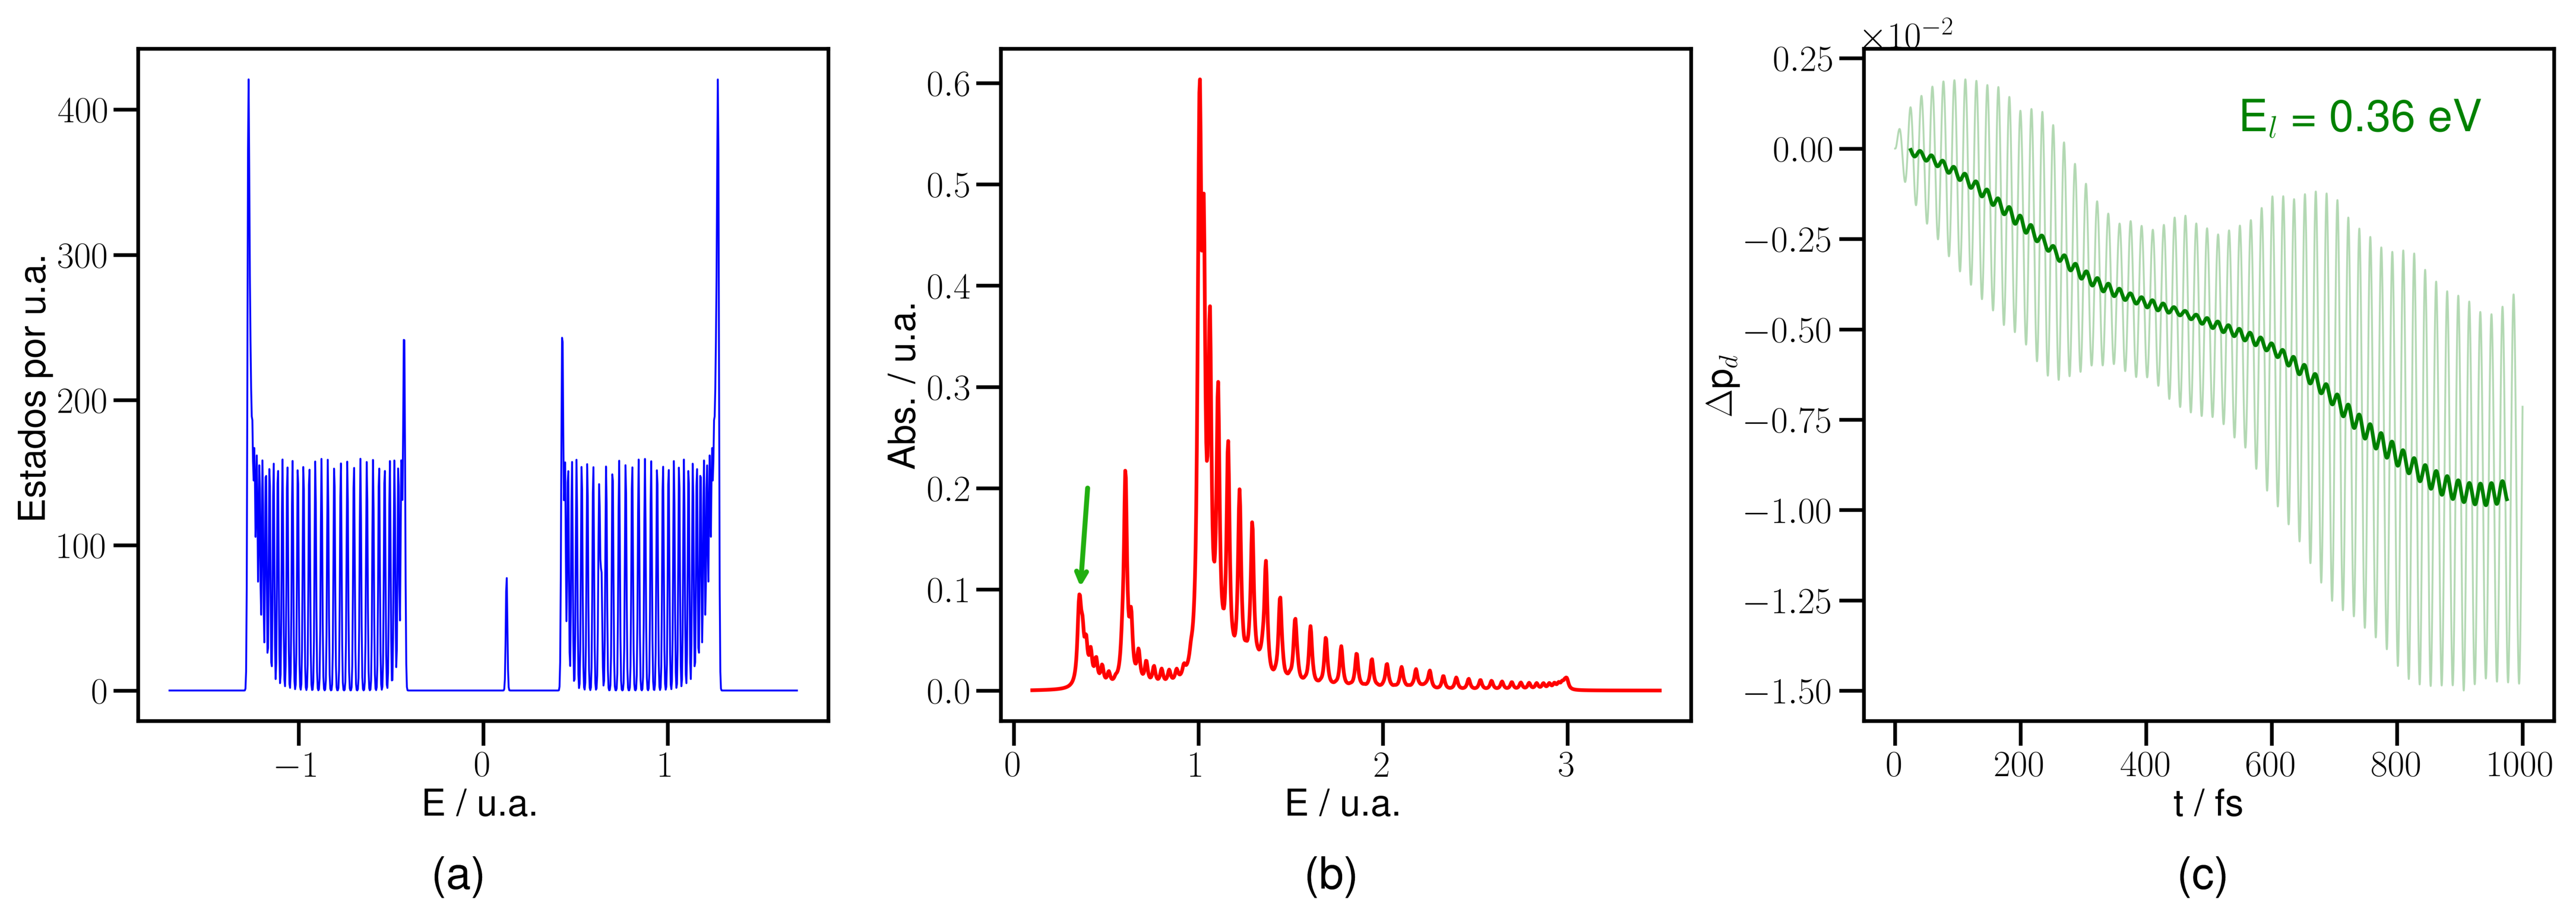
\includegraphics[height=4.8cm]{cap3/figs/fig_c_acople_ghost.eps}
 \caption{Sistema \textbf{(2-e)}. \textbf{(a)} DOS, \textbf{(b)} espectro de absorción y \textbf{(c)} diferencia de población en la diatómica respecto a la población inicial ($\Delta p_d$) en función del tiempo aplicando un campo electromagnético con energı́a $0.36$ u.a.}
 \label{2-e}
\end{figure}


La figura \ref{2-e} presenta los gráficos que se obtuvieron de las simulaciones del sistema \textbf{2-e}. La DOS \textbf{(a)} de este complejo no muestra cambios con respecto a la DOS del sistema sin interacción \textbf{1-e} porque los estados de la molécula y del SC son los mismos a pesar del acoplamiento.


En el espectro del sistema acoplado \textbf{(b)} se observan, nuevamente, el pico y la banda que corresponden a la absorción de la diatómica y el SC respectivamente. No obstante, aparece una nueva banda de menor intensidad y de menor energía en relación a las otras bandas presentes, que indica la aparición de nuevas transiciones en el sistema debidas al acoplamiento. De acuerdo con el potencial electroquímico de los electrones en el sistema ($\mu=0.3$) y con la ubicación energética de la diatómica ($\epsilon= 0.45$), el HOMO cuenta con electrones disponibles para las transiciones. Los mismos pueden excitarse hacia el LUMO o hacia la BC, lo cual está permitido por el acoplamiento incorporado. La nueva transición posible que surge de acoplar la diatómica con el SC ocurre desde el HOMO a la BC del SC (H-C) y se observa en el espectro como una banda a $0.36$ u.a. 

La evolución temporal de $\Delta p_d$ a medida que se ilumina con un láser con la energía de transición H-C ($0.36$ u.a.) se muestra en \textbf{(c)}. Es importante aclarar que las oscilaciones rápidas que se observan en la carga corresponden al período de oscilación del láser. La población de electrones disminuye con el tiempo debido a la perturbación, indicando la inyección de electrones a través de un proceso directo, desde el HOMO a la BC. La disminución de $\Delta p_d$ indica la transferencia de carga desde la molécula al SC.

Los resultados señalan entonces que se puede observar transferencia de carga al iluminar el complejo acoplado con una energia menor a la excitación H-L y que ocurre en una sola etapa.


\begin{figure}[!htb]
 \centering
 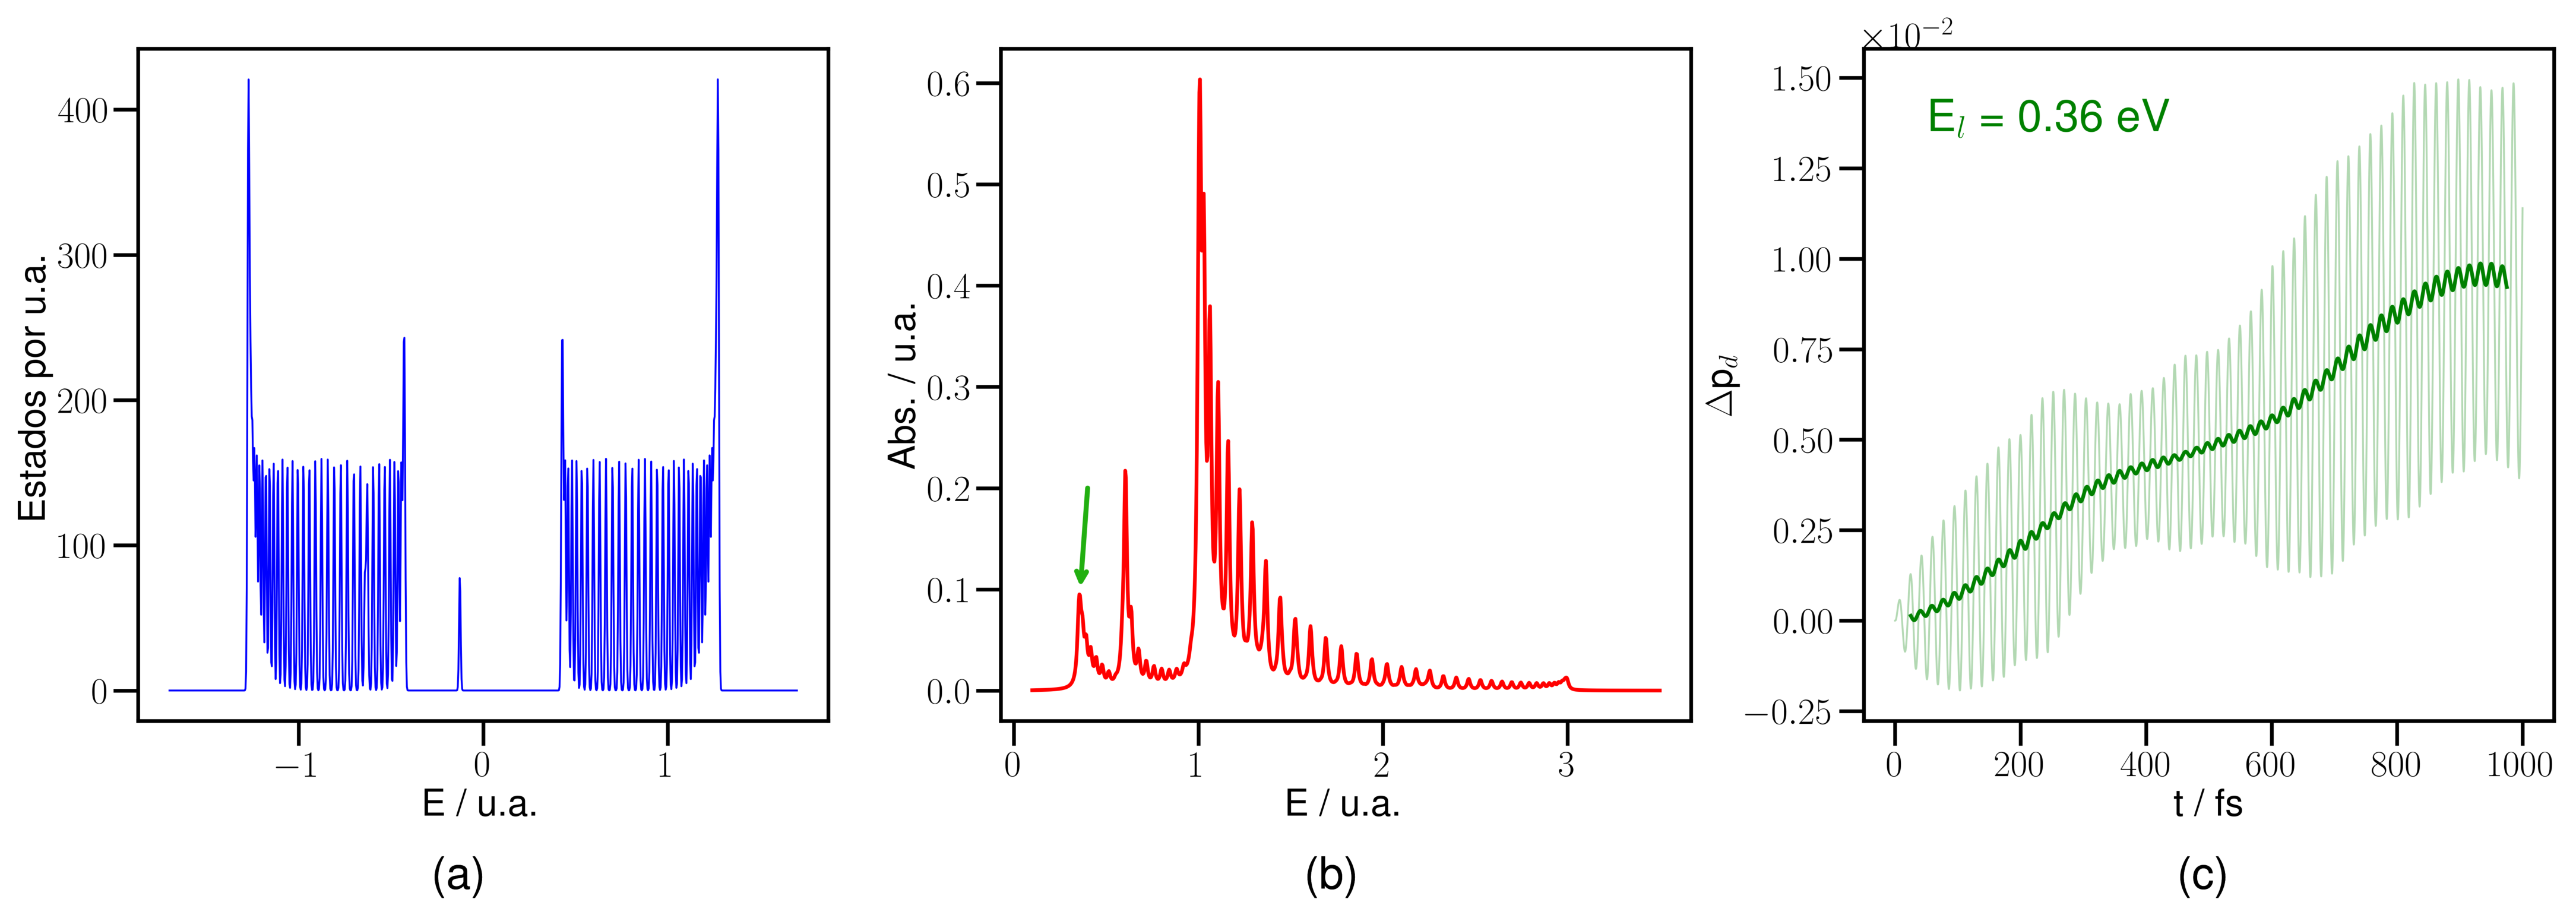
\includegraphics[height=4.8cm]{cap3/figs/fig_c_acople_ghost_hueco.eps}
 \caption{Sistema \textbf{(2-h)}. \textbf{(a)} DOS, \textbf{(b)} espectro de absorción y \textbf{(c)} diferencia de población en la diatómica respecto a la población inicial ($\Delta p_d$) en función del tiempo aplicando un campo electromagnético con energı́a $0.36$ u.a.}
 \label{2-h}
\end{figure}

La figura \ref{2-h} presenta los gráficos que se obtuvieron de las simulaciones del sistema \textbf{2-h}. La DOS \textbf{(a)} tampoco presenta cambios con respecto a la DOS del sistema no acoplado \textbf{1-h}. El espectro de absorción \textbf{(b)} se muestra idéntico al espectro del complejo \textbf{2-e} (ver figura \ref{2-e} \textbf{(b)}) y se debe a la simetría del modelo. Sin embargo, en este sistema, la banda a $0.36$ u.a. corresponde a transiciones que ocurren desde la BV del SC al HOMO de la molécula (V-H), lo cual se puede ver reflejado en el gráfico de $\Delta p_d$ en función del tiempo (ver figura \ref{2-h}\textbf{(c)}) al iluminar el complejo a $0.36$ u.a. La población de electrones aumenta con el tiempo, indicando la transferencia de carga desde el SC a la molécula, es decir en dirección opuesta al sistema \textbf{2-e}. La inyección de electrones al HOMO genera cargas positivas o huecos en el SC.

\subsubsection{Variación del acoplamiento}

Para que se logre una transferencia electrónica efectiva debe haber un buen acoplamiento electrónico entre los orbitales electrónicos del sensibilizador y la BC o BV del SC. Con la finalidad de explorar los efectos de los distintos grados de acoplamiento entre la molécula y el SC se analizaron complejos con $\gamma = 0$, $\gamma = 0.02$, $\gamma = 0.05$ y $\gamma = 0.1$ manteniendo $\epsilon=0.45$ y $\mu=0.30$ constantes, tal como muestra la figura \ref{2-e-g-t}.

\begin{figure}[!htb]
 \centering
 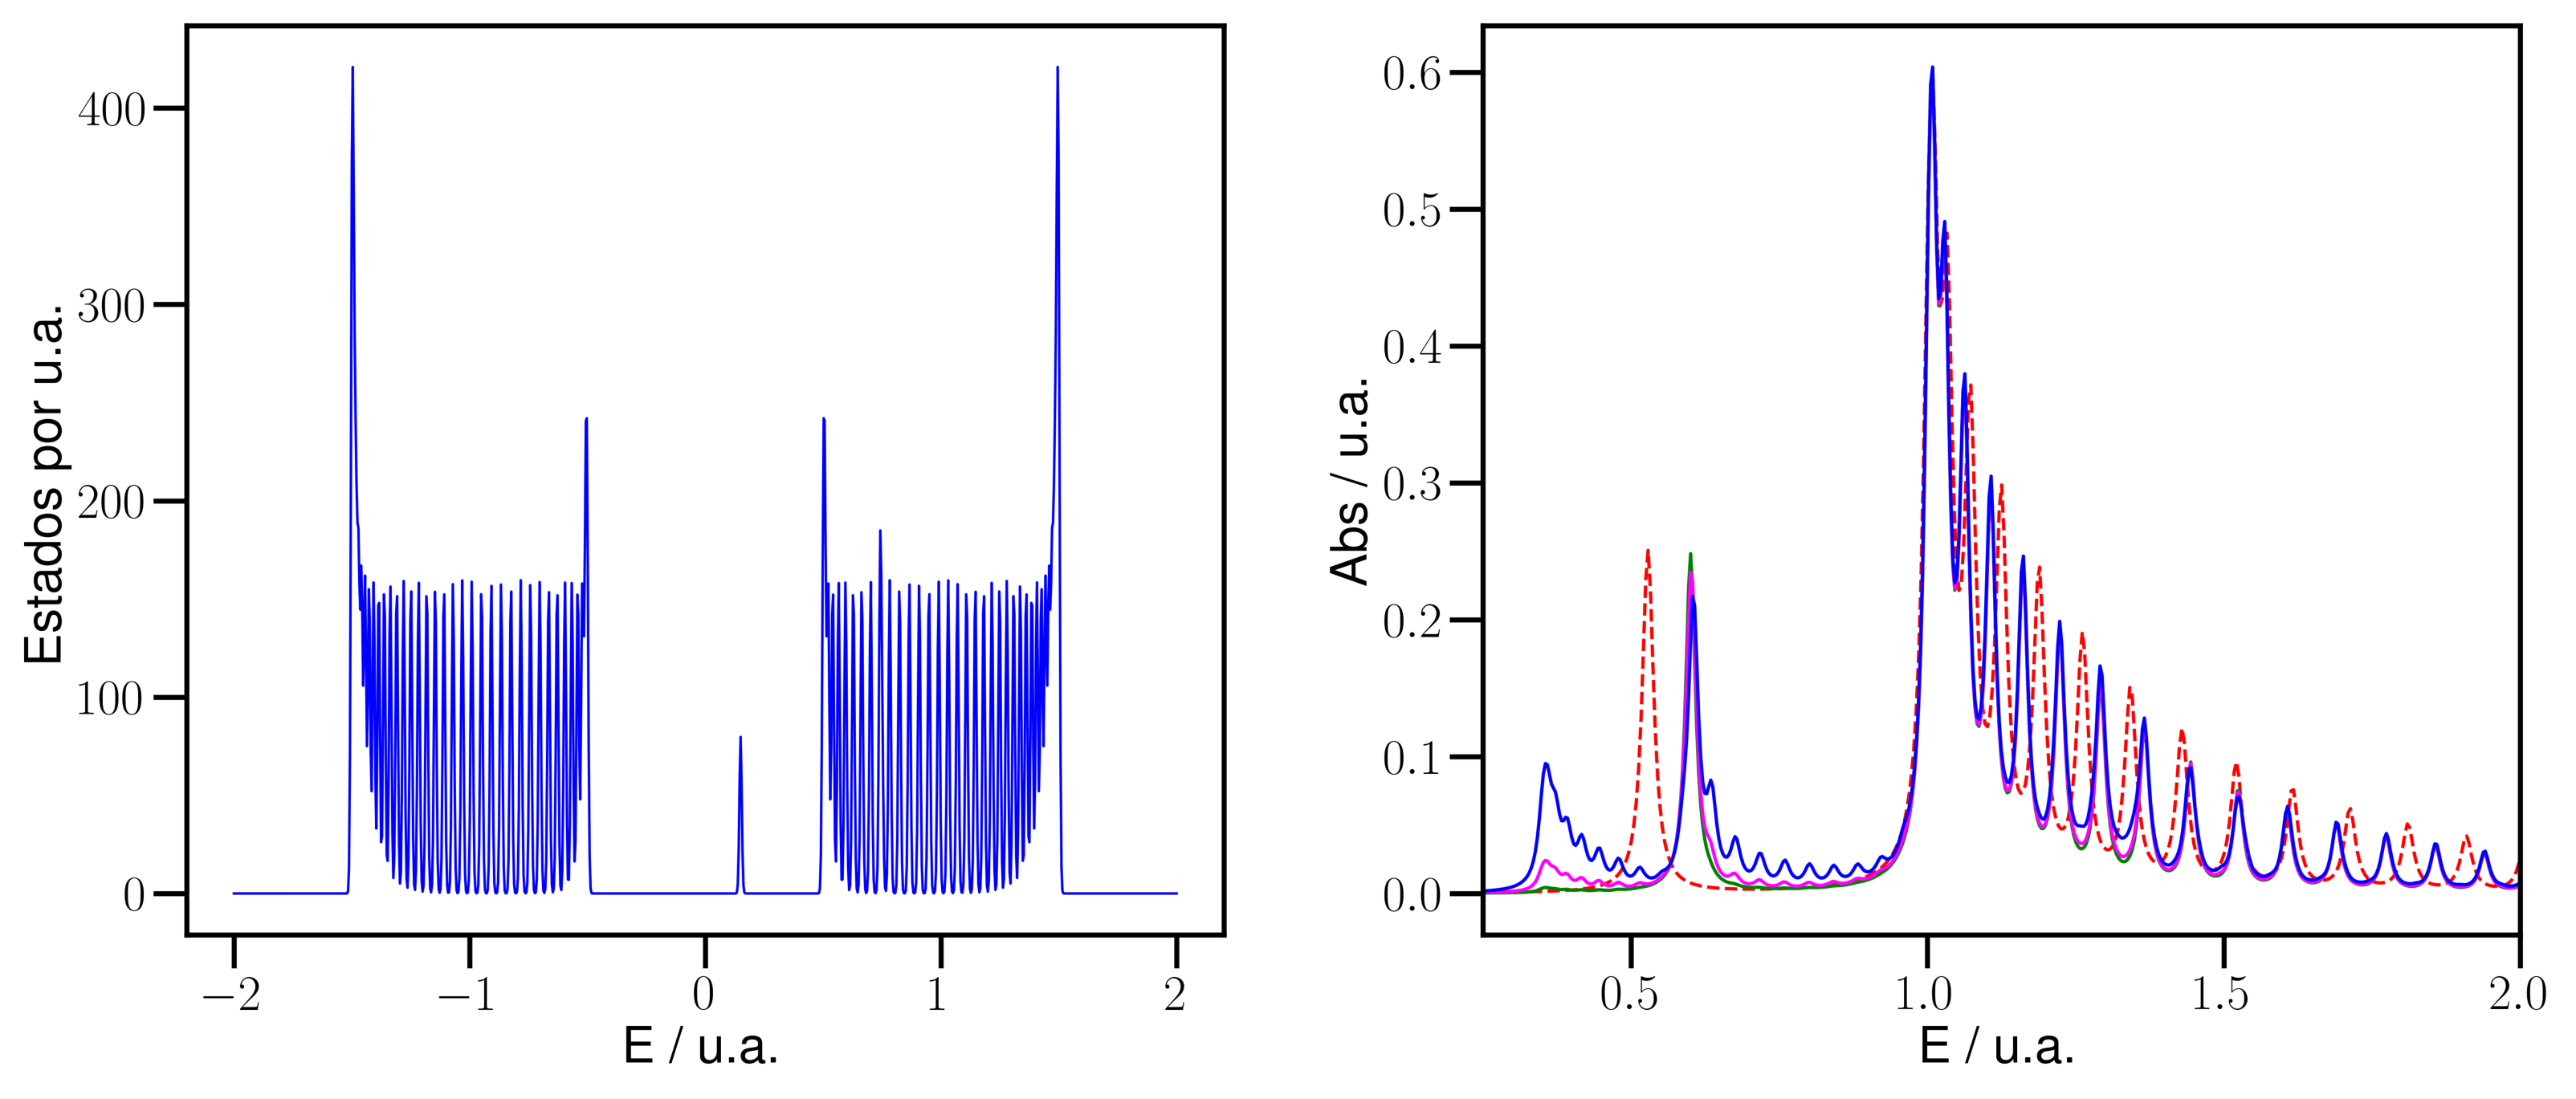
\includegraphics[height=5cm]{cap3/figs/fig_gamas_todo.eps}
 \caption{\textbf{(Izquierda)} DOS y \textbf{(derecha)} espectros de absorción para distintos acoplamientos: $\gamma = 0$, $\gamma = 0.02$, $\gamma = 0.05$ y $\gamma = 0.1$ utilizando $\epsilon=0.45$ y $\mu=0.3$ como parámetros fijos.}
 \label{2-e-g-t}
\end{figure}


\begin{figure}[!htb]
 \centering
 \includegraphics[height=4.3cm]{cap3/figs/fig_gamas_1.eps}
 \caption{Gráficos de \textbf{(a)} Espectro de absorción para distintos $\gamma$ y $\Delta p_d$ en función del tiempo aplicando un campo electromagnético con energı́a $0.36$ u.a. a complejos con distintos acoplamientos: \textbf{(b)} $\gamma = 0.02$, \textbf{(c)} $\gamma = 0.05$ y \textbf{(d)} $\gamma = 0.1$ }
 \label{2-e-g}
\end{figure}

En la figura \ref{2-e-g} \textbf{(a)} se observa el espectro de absorción en el rango ($0.2-0.8$) u.a. para las distintas $\gamma$ seleccionadas. La incorporación del acoplamiento genera por un lado el corrimiento de la banda del colorante a mayores energías, de $0.54$ u.a. a $0.60$ u.a., y por otro la aparición de una nueva banda a $0.36$ u.a. A medida que $\gamma$ crece, la absorción de la molécula disminuye mientras que la absorción de la banda nueva aumenta. Simultáneamente se observa que ambas bandas, la del colorante y la nueva, se parecen cada vez más (en forma) a la banda del SC (ver figura \ref{2-e-g-t}), lo cual deriva del mayor acoplamiento entre los niveles electrónicos. Cuando se utiliza $\gamma = 0.02$ la absorción de la nueva banda es tan pequeña que se considera despreciable.  


En la figura \ref{2-e-g} \textbf{(b)}, \textbf{(c)} y \textbf{(d)} se muestran los gráficos de $\Delta p_d$ en función del tiempo cuando se iluminan los complejos con un láser continuo sintonizado con la energía de la nueva banda ($0.36$ u.a.). En primer lugar se muestra que $\Delta p_d$ aumenta un orden de magnitud a medida que las constantes de acoplamiento crecen. En complejos con acoplamientos menores, como por ejemplo \textbf{(b)}, la transferencia de carga mediante el mecanismo directo es muy pequeña y por ende la contribución a la transferencia de carga total también es pequeña. Sin embargo, la inyección de electrones en la BC también puede ocurrir mediante otro tipo de mecanismo, es decir, la excitación H-L de la molécula y luego la introducción de los electrones en la BC. En la figura \ref{acople_chico} se observa que los valores de $\Delta p_d$ al iluminar con la energía de la molécula o $0.60$ u.a. son mayores con respecto a la iluminación a $0.36$ u.a. Con estos resultados podemos decir que la transferencia ocurre preferentemente mediante un mecanismo indirecto o en 2 etapas. 

\begin{figure}[!htb]
 \centering
 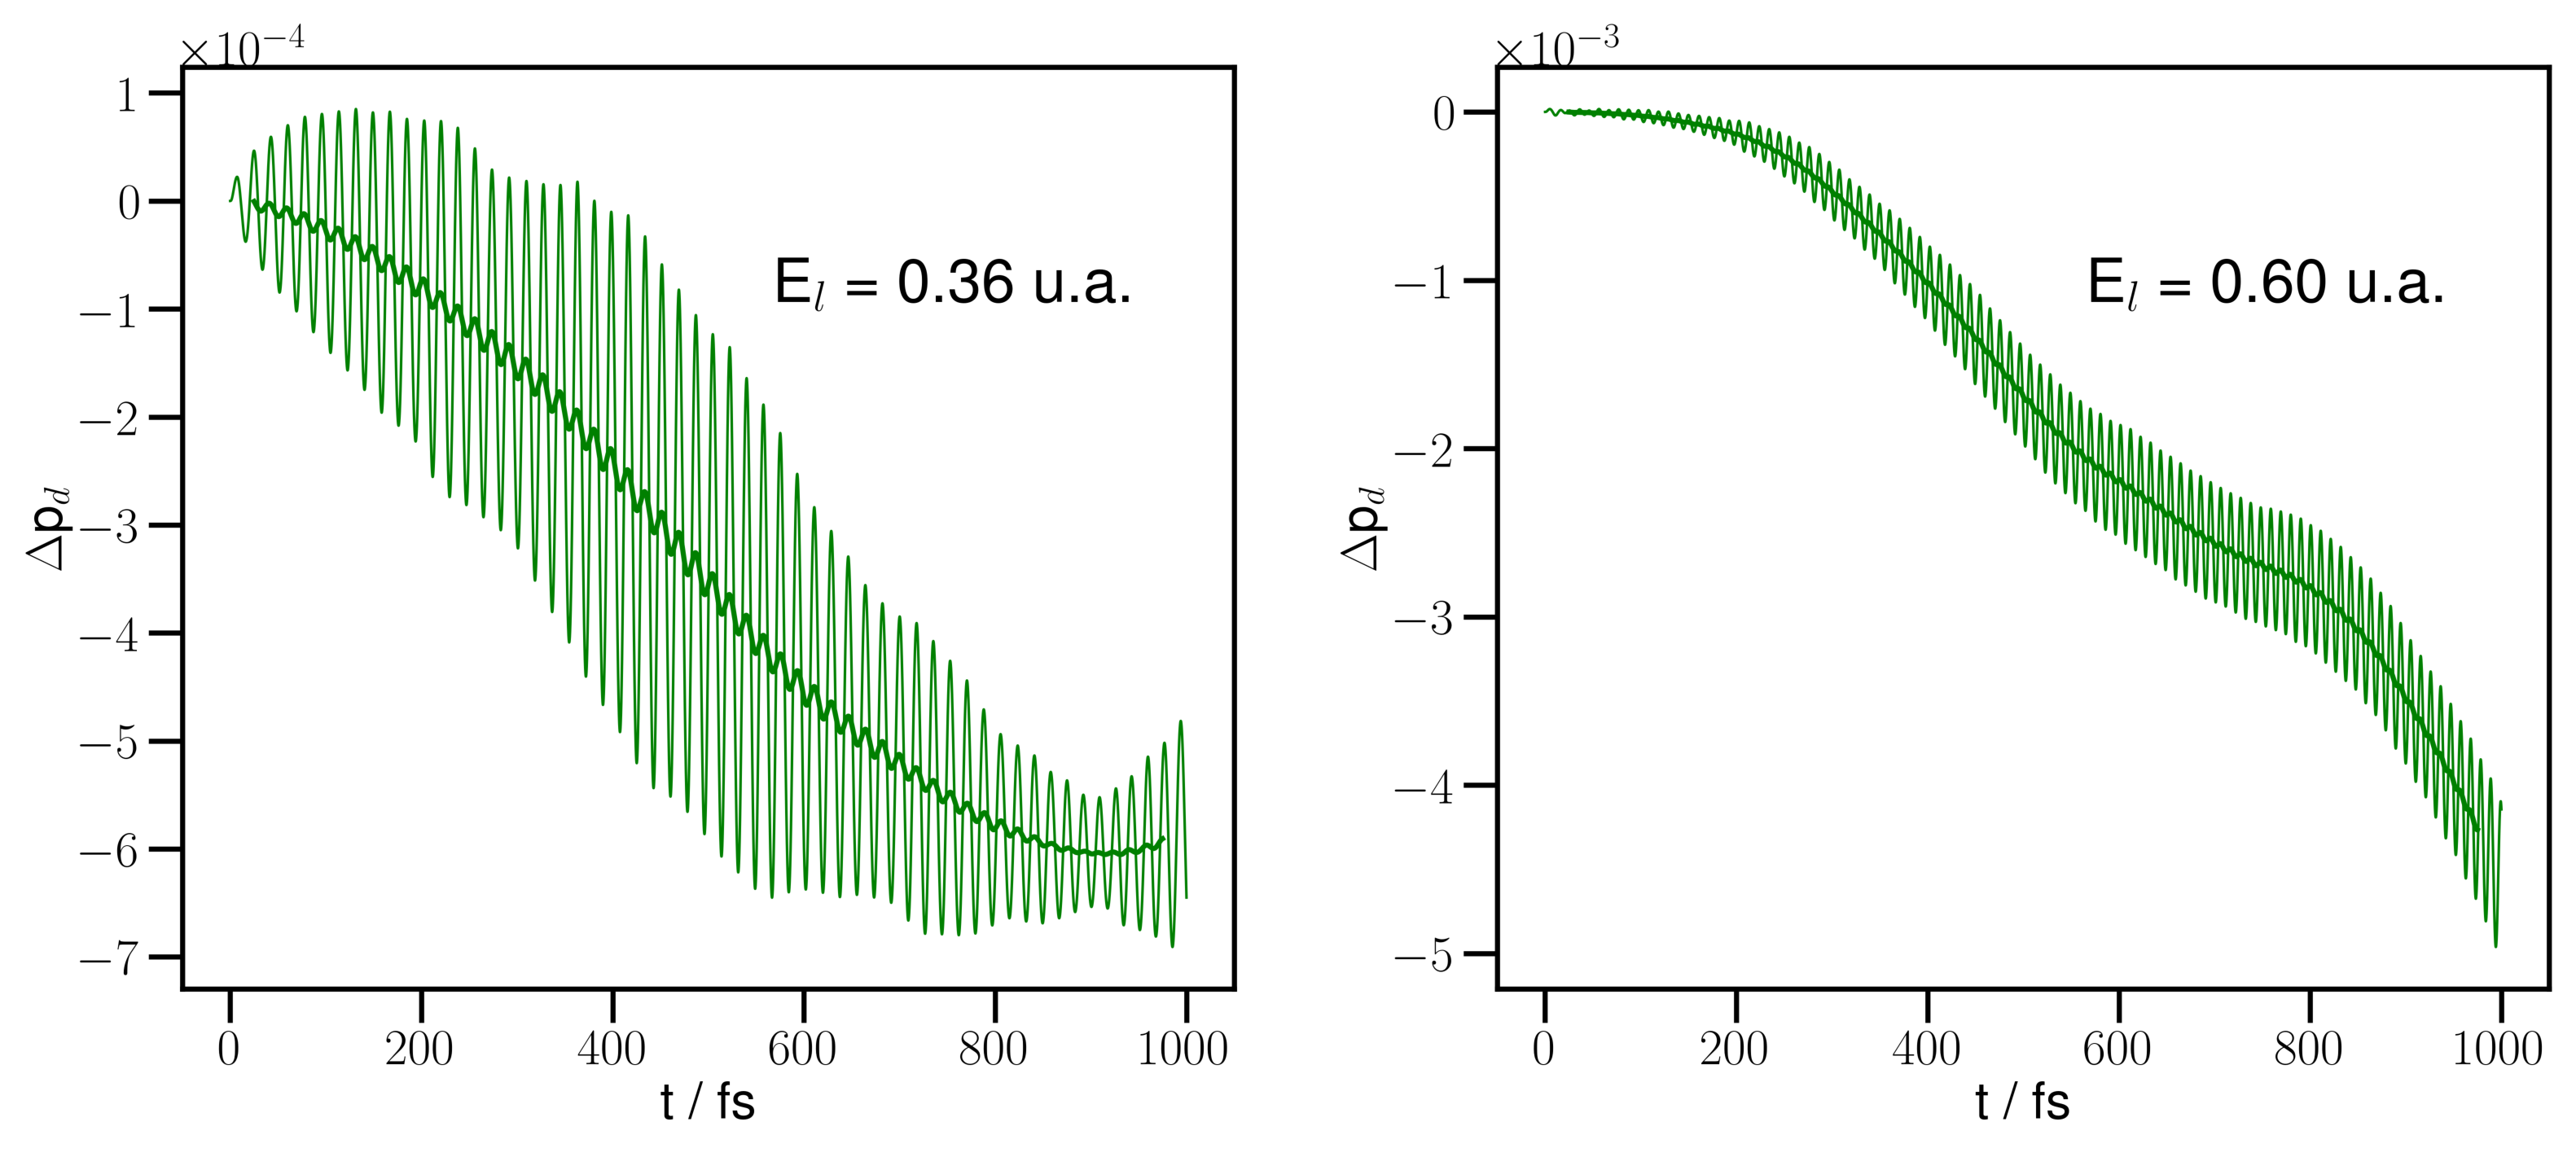
\includegraphics[height=4cm]{cap3/figs/acople_bajo.eps}
 \caption{$\Delta p_d$ en función del tiempo aplicando un campo electromagnético con energı́a $0.36$ u.a. \textbf{(izquerda)} y $0.60$ u.a. \textbf{(derecha)} al complejo con acoplamientos bajo o $\gamma = 0.02$}
 \label{acople_chico}
\end{figure}


En complejos con acoplamientos mayores, como por ejemplo \textbf{(d)}, observamos transferencia de carga mediante el mecanismo directo al iluminar los complejos con una energía de $0.36$ u.a. o con la energía de la transición H-C. En la figura \ref{acople_alto} se observa que los valores de $\Delta p_d$ al aplicar un campo con la energía de la excitación H-C, son mayores con respecto a la transferencia que produce la iluminación con la energía de la excitación H-L. Sin embargo, esta última no es tan pequeña como para considerarla despreciable. Podemos decir entonces que en sistemas donde el acoplamiento es grande, los dos mecanismos, tanto directo como indirecto contribuyen en la transferencia de carga final. 


\begin{figure}[!htb]
 \centering
 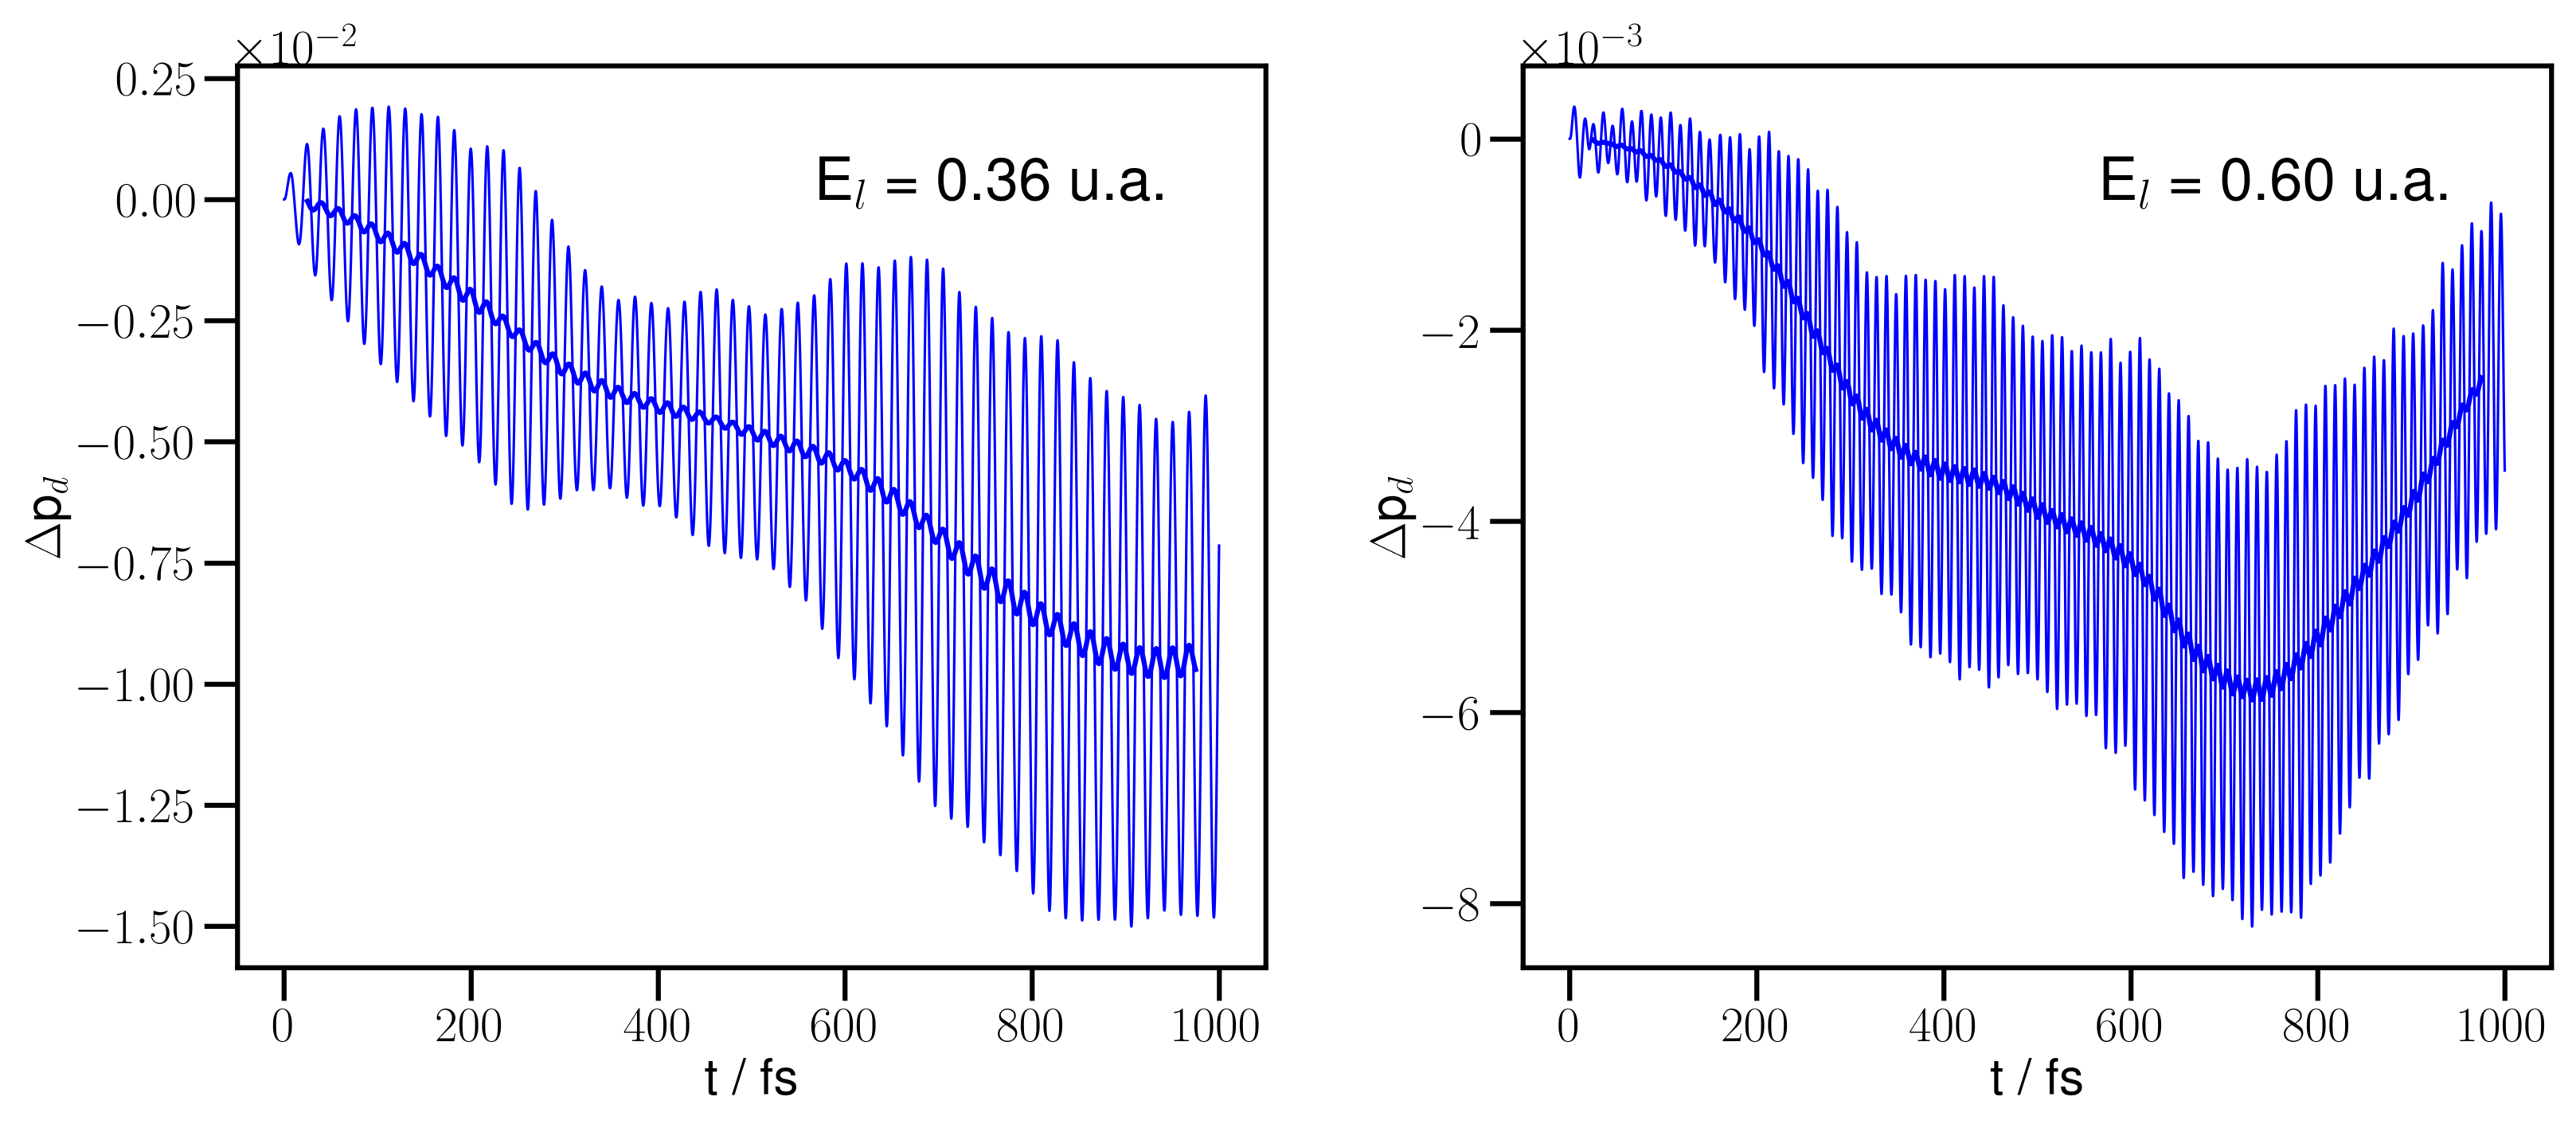
\includegraphics[height=4cm]{cap3/figs/acople_alto.eps}
 \caption{$\Delta p_d$ en función del tiempo aplicando un campo electromagnético con energı́a $0.36$ u.a. \textbf{(izquerda)} y $0.60$ u.a. \textbf{(derecha)} al complejo con acoplamientos bajo o $\gamma = 0.1$}
 \label{acople_alto}
\end{figure}
 
En última instancia consideramos complejos con las mismas constantes de acoplamiento utilizadas anteriormente, es decir, $\gamma = 0$, $\gamma = 0.02$, $\gamma = 0.05$ y $\gamma = 0.1$ pero esta vez con $\epsilon=-0.45$ y $\mu=-0.3$ constantes, tal como muestra la figura \ref{2-h-g}. Los gráficos de $\Delta p_d$ en función del tiempo \textbf{(b)}, \textbf{(c)} y \textbf{(d)} muestran la misma $\Delta p_d$ en valor absoluto en comparación a los gráficos de la figura \ref{2-e-g}, sin embargo en este caso,la inyección electrónica se produce desde el SC a la molécula.


\begin{figure}[!htb]
 \centering
 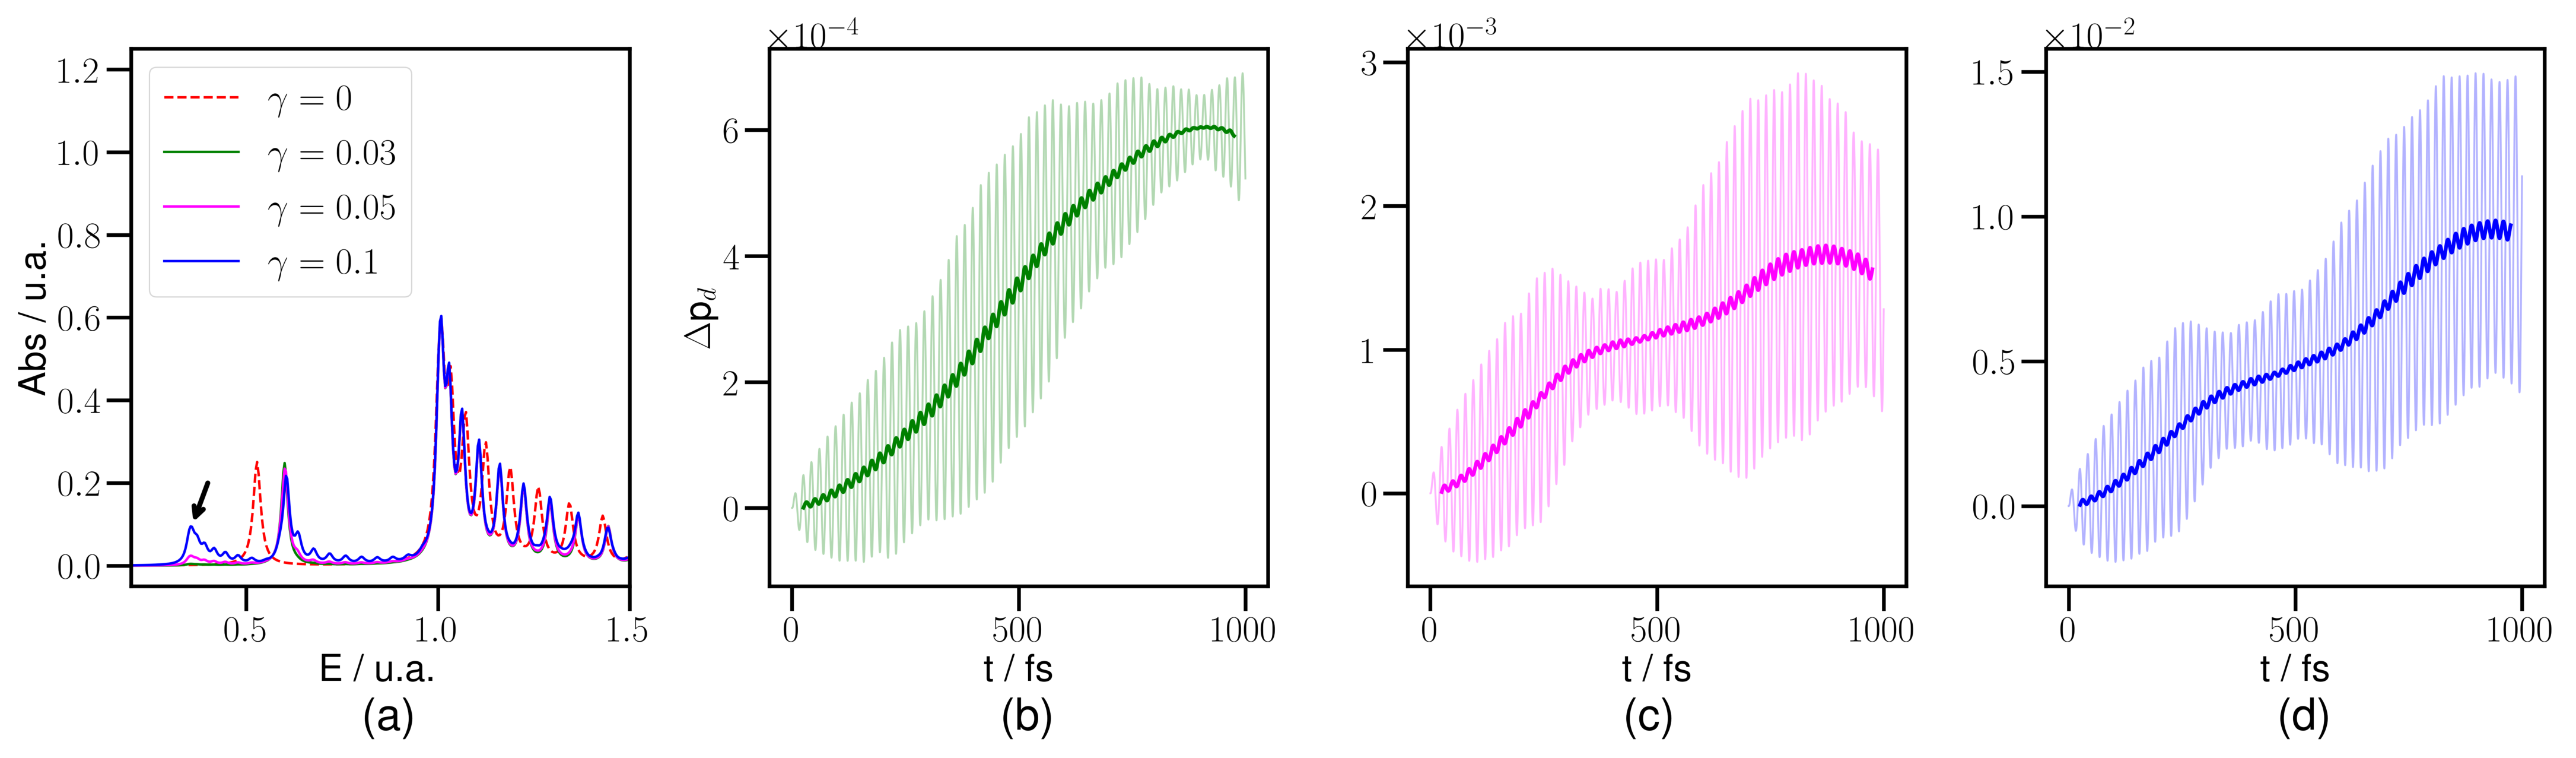
\includegraphics[height=4.3cm]{cap3/figs/fig_gamas_h.eps}
 \caption{Gráficos de \textbf{(a)} Espectro de absorción para distintos $\gamma$ y $\Delta p_d$ en función del tiempo aplicando un campo electromagnético con energı́a $0.36$ u.a. a complejos con distintos acoplamientos: \textbf{(b)} $\gamma = 0.02$, \textbf{(c)} $\gamma = 0.05$ y \textbf{(d)} $\gamma = 0.1$ utilizando $\epsilon=-0.45$ y $\mu=-0.3$ como parámetros fijos.}
 \label{2-h-g}
\end{figure}

\newpage


\section{Conclusiones}

 Los resultados obtenidos a lo largo del capítulo demuestran la efectividad del modelo para describir la dinámica electrónica del sistema molécula-SC bajo irradiación láser. Los cálculos para la DOS representan bien las BC y BV del SC separadas por un GAP y los orbitales H-L de la diatómica. Los espectros de absorción presentan claramente, en todos los casos, una banda que corresponde al SC con  una energía que comienza en 1 u.a. (energía del GAP) y un pico debido a la transición H-L. Cuando hay acoplamiento entre el anillo y la molécula aparece una nueva banda debido a nuevas transiciones posibles entre el SC y la molécula diatómica.  
 
 Cuando $\epsilon$ toma valores positivos, los orbitales de la diatómica se encuentran más cerca de la BC y por ende las transiciones menos energéticas son las que ocurren desde el HOMO a la BC. En este caso, la transferencia es electrónica. Cuando $\epsilon$ toma valores negativos, los orbitales de la diatómica se encuentran mas cerca de la BV y las transiciones menos energéticas son las transiciones que ocurren desde la BV al HOMO. En este caso la transferencia es de huecos ya que se genera una carga positiva en la BV. 
  
 Al variar la constante de acoplamiento se observó que cuando $\gamma$ es pequeña predomina el mecanismo de transferencia de carga indirecta y cuando $\gamma$ es grande predomina el mecanismo directo. Este comportamiento concuerda con lo observado anteriormente en el grupo, lo cual es otro indicio de que el modelo aunque sea simple representa bien el sistema DSSC y los procesos que ocurren en la misma.




 
